\documentclass[a4paper,14pt,oneside,openany]{memoir}

%%% Задаем поля, отступы и межстрочный интервал %%%

\usepackage[left=30mm, right=15mm, top=20mm, bottom=20mm]{geometry} % Пакет geometry с аргументами для определения полей
\pagestyle{plain} % Убираем стандарные для данного класса верхние колонтитулы с заголовком текущей главы, оставляем только номер страницы снизу по центру
\parindent=1.25cm % Абзацный отступ 1.25 см, приблизительно равно пяти знакам, как по ГОСТ
\usepackage{indentfirst} % Добавляем отступ к первому абзацу
%\linespread{1.3} % Межстрочный интервал (наиболее близко к вордовскому полуторному) - тут вместо этого используется команда OnehalfSpacing*

%%% Задаем языковые параметры и шрифт %%%

\usepackage[english, russian]{babel}                % Настройки для русского языка как основного в тексте
\babelfont[russian]{rm}{Times New Roman}                     % TMR в качестве базового roman-щрифта



%%% Задаем стиль заголовков и подзаголовков в тексте %%%

\setsecnumdepth{subsection} % Номера разделов считать до третьего уровня включительно, т.е. нумеруются только главы, секции, подсекции
\renewcommand*{\chapterheadstart}{} % Переопределяем команду, задающую отступ над заголовком, чтобы отступа не было
\renewcommand*{\printchaptername}{} % Переопределяем команду, печатающую слово "Глава", чтобы оно не печалось
%\renewcommand*{\printchapternum}{} % То же самое для номера главы - тут не надо, номер главы оставляем
\renewcommand*{\chapnumfont}{\normalfont\bfseries} % Меняем стиль шрифта для номера главы: нормальный размер, полужирный
\renewcommand*{\afterchapternum}{\hspace{1em}} % Меняем разделитель между номером главы и названием
\renewcommand*{\printchaptertitle}{\normalfont\bfseries\centering\MakeUppercase} % Меняем стиль написания для заголовка главы: нормальный размер, полужирный, центрированный, заглавными буквами
\setbeforesecskip{20pt} % Задаем отступ перед заголовком секции
\setaftersecskip{20pt} % Ставим такой же отступ после заголовка секции
\setsecheadstyle{\raggedright\normalfont\bfseries} % Меняем стиль написания для заголовка секции: выравнивание по правому краю без переносов, нормальный размер, полужирный
\setbeforesubsecskip{20pt} % Задаем отступ перед заголовком подсекции
\setaftersubsecskip{20pt} % Ставим такой же отступ после заголовка подсекции
\setsubsecheadstyle{\raggedright\normalfont\bfseries}  % Меняем стиль написания для заголовка подсекции: выравнивание по правому краю без переносов, нормальный размер, полужирный

%%% Задаем параметры оглавления %%%

\addto\captionsrussian{\renewcommand\contentsname{Содержание}} % Меняем слово "Оглавление" на "Содержание"
\setrmarg{2.55em plus1fil} % Запрещаем переносы слов в оглавлении
%\setlength{\cftbeforechapterskip}{0pt} % Эта команда убирает интервал между заголовками глав - тут не надо, так красивее смотрится
\renewcommand{\aftertoctitle}{\afterchaptertitle \vspace{-\cftbeforechapterskip}} % Делаем отступ между словом "Содержание" и первой строкой таким же, как у заголовков глав
%\renewcommand*{\chapternumberline}[1]{} % Делаем так, чтобы номер главы не печатался - тут не надо
\renewcommand*{\cftchapternumwidth}{1.5em} % Ставим подходящий по размеру разделитель между номером главы и самим заголовком
\renewcommand*{\cftchapterfont}{\normalfont\MakeUppercase} % Названия глав обычным шрифтом заглавными буквами
\renewcommand*{\cftchapterpagefont}{\normalfont} % Номера страниц обычным шрифтом
\renewcommand*{\cftchapterdotsep}{\cftdotsep} % Делаем точки до номера страницы после названий глав
\renewcommand*{\cftdotsep}{1} % Задаем расстояние между точками
\renewcommand*{\cftchapterleader}{\cftdotfill{\cftchapterdotsep}} % Делаем точки стандартной формы (по умолчанию они "жирные")
\maxtocdepth{subsection} % В оглавление попадают только разделы первыхтрех уровней: главы, секции и подсекции

%%% Выравнивание и переносы %%%

%% http://tex.stackexchange.com/questions/241343/what-is-the-meaning-of-fussy-sloppy-emergencystretch-tolerance-hbadness
%% http://www.latex-community.org/forum/viewtopic.php?p=70342#p70342
\tolerance 1414
\hbadness 1414
\emergencystretch 1.5em                             % В случае проблем регулировать в первую очередь
\hfuzz 0.3pt
\vfuzz \hfuzz
%\dbottom
%\sloppy                                            % Избавляемся от переполнений
\clubpenalty=10000                                  % Запрещаем разрыв страницы после первой строки абзаца
\widowpenalty=10000                                 % Запрещаем разрыв страницы после последней строки абзаца
\brokenpenalty=4991                                 % Ограничение на разрыв страницы, если строка заканчивается переносом

%%% Объясняем компилятору, какие буквы русского алфавита можно использовать в перечислениях (подрисунках и нумерованных списках) %%%
%%% По ГОСТ нельзя использовать буквы ё, з, й, о, ч, ь, ы, ъ %%%
%%% Здесь также переопределены заглавные буквы, хотя в принципе они в документе не используются %%%

\makeatletter
    \def\russian@Alph#1{\ifcase#1\or
       А\or Б\or В\or Г\or Д\or Е\or Ж\or
       И\or К\or Л\or М\or Н\or
       П\or Р\or С\or Т\or У\or Ф\or Х\or
       Ц\or Ш\or Щ\or Э\or Ю\or Я\else\xpg@ill@value{#1}{russian@Alph}\fi}
    \def\russian@alph#1{\ifcase#1\or
       а\or б\or в\or г\or д\or е\or ж\or
       и\or к\or л\or м\or н\or
       п\or р\or с\or т\or у\or ф\or х\or
       ц\or ш\or щ\or э\or ю\or я\else\xpg@ill@value{#1}{russian@alph}\fi}
\makeatother

%%% Задаем параметры оформления рисунков и таблиц %%%

\usepackage{graphicx, caption, subcaption} % Подгружаем пакеты для работы с графикой и настройки подписей
\graphicspath{{images/}} % Определяем папку с рисунками
\captionsetup[figure]{font=small, width=\textwidth, name=Рисунок, justification=centering} % Задаем параметры подписей к рисункам: маленький шрифт (в данном случае 12pt), ширина равна ширине текста, полнотекстовая надпись "Рисунок", выравнивание по центру
\captionsetup[subfigure]{font=small} % Индексы подрисунков а), б) и так далее тоже шрифтом 12pt (по умолчанию делает еще меньше)
\captionsetup[table]{singlelinecheck=false,font=small,width=\textwidth,justification=justified} % Задаем параметры подписей к таблицам: запрещаем переносы, маленький шрифт (в данном случае 12pt), ширина равна ширине текста, выравнивание по ширине
\captiondelim{ --- } % Разделителем между номером рисунка/таблицы и текстом в подписи является длинное тире
\setkeys{Gin}{width=\textwidth} % По умолчанию размер всех добавляемых рисунков будет подгоняться под ширину текста
\renewcommand{\thesubfigure}{\asbuk{subfigure}} % Нумерация подрисунков строчными буквами кириллицы
%\setlength{\abovecaptionskip}{0pt} % Отбивка над подписью - тут не меняем
%\setlength{\belowcaptionskip}{0pt} % Отбивка под подписью - тут не меняем
\usepackage[section]{placeins} % Объекты типа float (рисунки/таблицы) не вылезают за границы секциии, в которой они объявлены

%%% Задаем параметры ссылок и гиперссылок %%% 

\usepackage{hyperref}                               % Подгружаем нужный пакет
\hypersetup{
    colorlinks=true,                                % Все ссылки и гиперссылки цветные
    linktoc=all,                                    % В оглавлении ссылки подключатся для всех отображаемых уровней
    linktocpage=true,                               % Ссылка - только номер страницы, а не весь заголовок (так выглядит аккуратнее)
    linkcolor=red,                                  % Цвет ссылок и гиперссылок - красный
    citecolor=red                                   % Цвет цитировний - красный
}

%%% Настраиваем отображение списков %%%

\usepackage{enumitem}                               % Подгружаем пакет для гибкой настройки списков
\renewcommand*{\labelitemi}{\normalfont{--}}        % В ненумерованных списках для пунктов используем короткое тире
\makeatletter
    \AddEnumerateCounter{\asbuk}{\russian@alph}     % Объясняем пакету enumitem, как использовать asbuk
\makeatother
\renewcommand{\labelenumii}{\asbuk{enumii})}        % Кириллица для второго уровня нумерации
\renewcommand{\labelenumiii}{\arabic{enumiii})}     % Арабские цифры для третьего уровня нумерации
\setlist{noitemsep, leftmargin=*}                   % Убираем интервалы между пунками одного уровня в списке
\setlist[1]{labelindent=\parindent}                 % Отступ у пунктов списка равен абзацному отступу
\setlist[2]{leftmargin=\parindent}                  % Плюс еще один такой же отступ для следующего уровня
\setlist[3]{leftmargin=\parindent}                  % И еще один для третьего уровня

%%% Счетчики для нумерации объектов %%%

\counterwithout{figure}{chapter}                    % Сквозная нумерация рисунков по документу
\counterwithout{equation}{chapter}                  % Сквозная нумерация математических выражений по документу
\counterwithout{table}{chapter}                     % Сквозная нумерация таблиц по документу

%%% Реализация библиографии пакетами biblatex и biblatex-gost с использованием движка biber %%%

\usepackage{csquotes} % Пакет для оформления сложных блоков цитирования (biblatex рекомендует его подключать)
\usepackage[%
backend=biber,                                      % Движок
bibencoding=utf8,                                   % Кодировка bib-файла
sorting=none,                                       % Настройка сортировки списка литературы
style=gost-numeric,                                 % Стиль цитирования и библиографии по ГОСТ
language=auto,                                      % Язык для каждой библиографической записи задается отдельно
autolang=other,                                     % Поддержка многоязычной библиографии
sortcites=true,                                     % Если в квадратных скобках несколько ссылок, то отображаться будут отсортированно
movenames=false,                                    % Не перемещать имена, они всегда в начале библиографической записи
maxnames=5,                                         % Максимальное отображаемое число авторов
minnames=3,                                         % До скольки сокращать число авторов, если их больше максимума
doi=false,                                          % Не отображать ссылки на DOI
isbn=false,                                         % Не показывать ISBN, ISSN, ISRN
]{biblatex}[2016/09/17]
\DeclareDelimFormat{bibinitdelim}{}                 % Убираем пробел между инициалами (Иванов И.И. вместо Иванов И. И.)
\addbibresource{bibl.bib}                           % Определяем файл с библиографией

%%% Скрипт, который автоматически подбирает язык (и, следовательно, формат) для каждой библиографической записи %%%
%%% Если в названии работы есть кириллица - меняем значение поля langid на russian %%%
%%% Все оставшиеся пустые места в поле langid заменяем на english %%%

\DeclareSourcemap{
  \maps[datatype=bibtex]{
    \map{
        \step[fieldsource=title, match=\regexp{^\P{Cyrillic}*\p{Cyrillic}.*}, final]
        \step[fieldset=langid, fieldvalue={russian}]
    }
    \map{
        \step[fieldset=langid, fieldvalue={english}]
    }
  }
}

%%% Прочие пакеты для расширения функционала %%%

\usepackage{longtable,ltcaption}                    % Длинные таблицы
\usepackage{multirow,makecell}                      % Улучшенное форматирование таблиц
\usepackage{booktabs}                               % Еще один пакет для красивых таблиц
\usepackage{soulutf8}                               % Поддержка переносоустойчивых подчёркиваний и зачёркиваний
\usepackage{icomma}                                 % Запятая в десятичных дробях
\usepackage{hyphenat}                               % Для красивых переносов
\usepackage{textcomp}                               % Поддержка "сложных" печатных символов типа значков иены, копирайта и т.д.
\usepackage[version=4]{mhchem}                      % Красивые химические уравнения
\usepackage{amsmath}                                % Усовершенствование отображения математических выражений
\usepackage{listings} 

%%% Вставляем по очереди все содержательные части документа %%%

\begin{document}

\thispagestyle{empty}

\begin{center}
    МИНИСТЕРСТВО ЦИФРОВОГО РАЗВИТИЯ, СВЯЗИ И МАССОВЫХ КОММУНИКАЦИЙ \\ РОССИЙСКОЙ ФЕДЕРАЦИИ

    \vspace{20pt}

    Федеральное государственное бюджетное образовательное учреждение  \\  высшего образования \\
    "<Сибирский государственный университет телекоммуникаций и информатики"> \\

    \vspace{20pt}

    Кафедра телекоммуникационных систем и вычислительных средств \\  (ТС и ВС)
\end{center}

\vfill

\begin{center}
    РГР \\  
    по дисциплине \\
    \textit{"<Визуальное програмироавние">}

    \vspace{20pt}

    по теме: \\
    \uppercase{Разработка Медиа-плеера на Android с использованием Jetpack Compose}
\end{center}

\vfill

    \noindent Студент: \\
    \textit{Группа ИА-331 \hfill С.Х. Иргит}

    \vspace{20pt}

    \noindent Предподаватель: \\
    \textit{Старший преподаватель \hfill Р.В. Ахпашев}

\vfill

\begin{center}
    Новосибирск 2025 г.
\end{center}                                     % Титульник

\newpage % Переходим на новую страницу
\setcounter{page}{2} % Начинаем считать номера страниц со второй
\OnehalfSpacing* % Задаем полуторный интервал текста (в титульнике одинарный, поэтому команда стоит после него)

\tableofcontents*                                   % Автособираемое оглавление

\chapter{Введение}
 Современные мобильные устройства предоставляют широкие возможности для обработки мультимедийной информации.
  Аудио и видео являются важной частью пользовательского опыта, особенно в эпоху постоянной доступности потоковых и локальных медиа.
   Одной из базовых задач является воспроизведение аудиофайлов, что реализуется с помощью медиаплееров.

Актуальность темы обусловлена тем, что с каждым годом растёт количество пользователей Android, а спрос на качественные и функциональные мультимедийные приложения не снижается.
 Поэтому рассмотрение практической реализации аудиоплеера — это полезная задача как с точки зрения обучения, так и с точки зрения создания реального продукта.

В работе рассматривается создание простого медиаплеера с графическим интерфейсом на основе Jetpack Compose — современного инструмента для UI-разработки от Google. 
Приложение позволяет воспроизводить локальные аудиофайлы, переключаться между треками и управлять воспроизведением.
                                     % Введение
\chapter{Постановка задачи}

\section{Цель работы}

Целью данной работы является разработка мобильного приложения — медиа плеера , реализованного на языке Kotlin. Интерфейс создаётся с помощью Jetpack Compose \cite{android-compose}.

\section{Задачи}
Реализовать основные функции медиа плеера: воспроизведение аудиофайлов, навигация по плейлисту, пауза, переход к следующему/предыдущему треку, отображение информации о треке.
                                     % Первая глава
\chapter{Теоретическая часть}

\subsection{Jetpack Compose}
Jetpack Compose представляет собой декларативный подход к разработке пользовательских интерфейсов.
В отличие от традиционного XML, в Compose UI описывается c помощью функций на Kotlin \cite{kotlin-doc}.
Это упрощает разработку и позволяет избежать избыточности кода.
Например, элемент интерфейса может быть создан как простая функция:

\begin{lstlisting}
@Composable
fun Greeting(name: String) {
    Text(text = "Hello $name!")
}
\end{lstlisting}


\subsection{MediaPlayer API}
Для воспроизведения аудио в Android используется класс \texttt{MediaPlayer}\cite{android-mediaplayer}. Он предоставляет следующие возможности:
\begin{itemize}
  \item Загрузка локальных и удалённых аудиофайлов;
  \item Поддержка различных форматов (MP3, WAV, OGG и др.);
  \item Управление воспроизведением (пауза, стоп, перемотка);
  \item Работа в фоновом режиме.
\end{itemize}

Пример использования MediaPlayer:

\begin{lstlisting}
val player = MediaPlayer()
player.setDataSource("path/to/file.mp3")
player.prepare()
player.start()
\end{lstlisting}

\subsection{Система разрешений в Android}

Начиная с Android 6.0 (API 23), система безопасности требует запроса разрешений во время выполнения (runtime permissions). Для доступа к файлам, расположенным во внешнем хранилище, необходимо явно запрашивать разрешение у пользователя. Android разделяет разрешения на два типа: обычные (normal) и опасные (dangerous). Чтение медиафайлов относится ко второму типу.

С Android 13 (API 33) были введены новые отдельные разрешения, включая \texttt{READ\_MEDIA\_AUDIO}\cite{android-permissions}, позволяющее приложению читать только аудиофайлы. Это позволяет более точно контролировать доступ приложений к пользовательским данным.

В Jetpack Compose для запроса разрешения используется специальный механизм:

\begin{lstlisting}
val launcher = rememberLauncherForActivityResult(
    ActivityResultContracts.RequestPermission()
) { isGranted ->
    if (isGranted) {
        // Разрешение получено
    }
}
\end{lstlisting}

\subsection{Работа с состоянием в Compose}

Jetpack Compose использует реактивную модель состояния. Это означает, что UI автоматически обновляется при изменении состояния. Для хранения состояния используется API \texttt{remember} и \texttt{mutableStateOf}:

\begin{lstlisting}
var isPlaying by remember { mutableStateOf(false) }

Button(onClick = { isPlaying = !isPlaying }) {
    Text(if (isPlaying) "Pause" else "Play")
}
\end{lstlisting}

Состояния в Compose позволяют создавать динамические и отзывчивые интерфейсы без необходимости ручного обновления UI-элементов.

\subsection{Обработка жизненного цикла и ресурсов}

При работе с мультимедиа важно учитывать жизненный цикл активности. Объекты, такие как \texttt{MediaPlayer}, требуют ручного освобождения ресурсов во избежание утечек памяти. Compose предоставляет функцию \texttt{DisposableEffect}, которая позволяет управлять ресурсами:

\begin{lstlisting}
DisposableEffect(Unit) {
    onDispose {
        player.release()
    }
}
\end{lstlisting}

Это особенно полезно для компонентов, которые не управляются фреймворком напрямую, как в случае с Java- или Android-классами.

\subsection{Архитектурные подходы: MVVM}

Несмотря на то, что демонстрационное приложение реализовано в одном файле, для более масштабных проектов рекомендуется использовать архитектурный паттерн MVVM (Model-View-ViewModel). В нём:

\begin{itemize}
  \item \textbf{Model} — содержит бизнес-логику и доступ к данным (например, загрузка аудиофайлов);
  \item \textbf{ViewModel} — содержит состояние UI и бизнес-логику, обрабатывает события;
  \item \textbf{View} — Jetpack Compose-компоненты, подписанные на данные ViewModel.
\end{itemize}

Jetpack предоставляет библиотеку \texttt{androidx.lifecycle.viewmodel.compose.viewModel}, которая позволяет интегрировать ViewModel в Compose-приложения.

\subsection{Преимущества использования Jetpack Compose}

Jetpack Compose обладает рядом преимуществ по сравнению с традиционным подходом через XML:

\begin{itemize}
  \item Более простая и лаконичная запись интерфейсов;
  \item Возможность полной декларативности и реактивности;
  \item Отличная поддержка LiveData и Flow;
  \item Интеграция с архитектурными компонентами Android;
  \item Улучшенная совместимость с Kotlin.
\end{itemize}                                     % Вторая глава
\chapter{Практическая часть}
\section{Анализ и структура реализации музыкального плеера}
Проект состоит из одной основной активности и одного основного компонента для интерфейса.

\subsection{Структура проекта}

В проекте определена одна активность — \texttt{MediaPlayerActivity}, которая служит точкой входа и отвечает за запуск пользовательского интерфейса с помощью функции \texttt{setContent}. Внутри вызывается основная компонуемая функция \texttt{MusicLibraryUI}, реализующая весь интерфейс и логику плеера.

\subsection{Функция интерфейса MusicLibraryUI}

Функция \texttt{MusicLibraryUI} выполняет ключевые задачи приложения:

\begin{itemize}
  \item Запрашивает у пользователя разрешение на чтение медиафайлов;
  \item Загружает аудиофайлы из папки \texttt{Music} во внешнем хранилище;
  \item Отображает список доступных треков с помощью компонента \texttt{LazyColumn};
  \item Управляет воспроизведением треков с помощью \texttt{MediaPlayer};
  \item Следит за состоянием плеера и обновляет интерфейс (позиция, длительность и т.д.).
\end{itemize}

\subsection{Запрос разрешений}

Для корректной работы с файловой системой необходимо запросить соответствующие разрешения у пользователя. В зависимости от версии Android используются:

\begin{itemize}
    \item \texttt{READ\_MEDIA\_AUDIO} --- начиная с Android 13 (API 33);
    \item \texttt{READ\_EXTERNAL\_STORAGE} --- для Android 12 и ниже.
\end{itemize}

Разрешения запрашиваются через механизм \texttt{rememberLauncherForActivityResult} из Compose API.

\subsection{Загрузка аудиофайлов}

Файлы с расширениями \texttt{.mp3}, \texttt{.wav}, \texttt{.ogg} загружаются с помощью функции \texttt{loadAudioFiles}, которая ищет их в стандартной папке \texttt{Environment.DIRECTORY\_MUSIC}.

\subsection{Управление воспроизведением}

Воспроизведение реализовано с помощью Android API \texttt{MediaPlayer}. Функция \texttt{playTrack(index)} отвечает за выбор и воспроизведение трека. Также предусмотрены следующие элементы управления:

\begin{itemize}
    \item Переключение на следующий и предыдущий трек;
    \item Кнопка воспроизведения и паузы;
    \item Отображение текущей позиции воспроизведения и полной длительности трека.
\end{itemize}

Состояние обновляется в режиме реального времени с помощью корутин и реактивных состояний Compose.

\subsection{Пользовательский интерфейс}

Интерфейс построен на компонентах Jetpack Compose: \texttt{Column}, \texttt{LazyColumn}, \texttt{ListItem}, \texttt{IconButton}. При выборе трека пользователь видит его название, а также может управлять воспроизведением через удобный набор иконок. Приложение динамически обновляет отображаемую информацию в зависимости от выбранного трека и текущего состояния плеера.

\newpage                                     % Третья глава
\chapter{Заключение}
Разработка медиаплеера на Android позволила на практике освоить ключевые концепции платформы, включая работу с разрешениями, пользовательским интерфейсом и воспроизведением медиа.
Применение Jetpack Compose упростило реализацию UI, сделав код более читаемым и гибким.
Созданное приложение может стать базой для более сложного медиаплеера, поддерживающего плейлисты, обложки, работу в фоне и другие функции.
Работа имеет практическую ценность как учебный проект, демонстрирующий современные подходы к мобильной разработке.

\newpage                                     % Четвертая глава
\chapter*{Приложение}

\begin{figure}[h] % h – размещение "здесь"
    \centering
    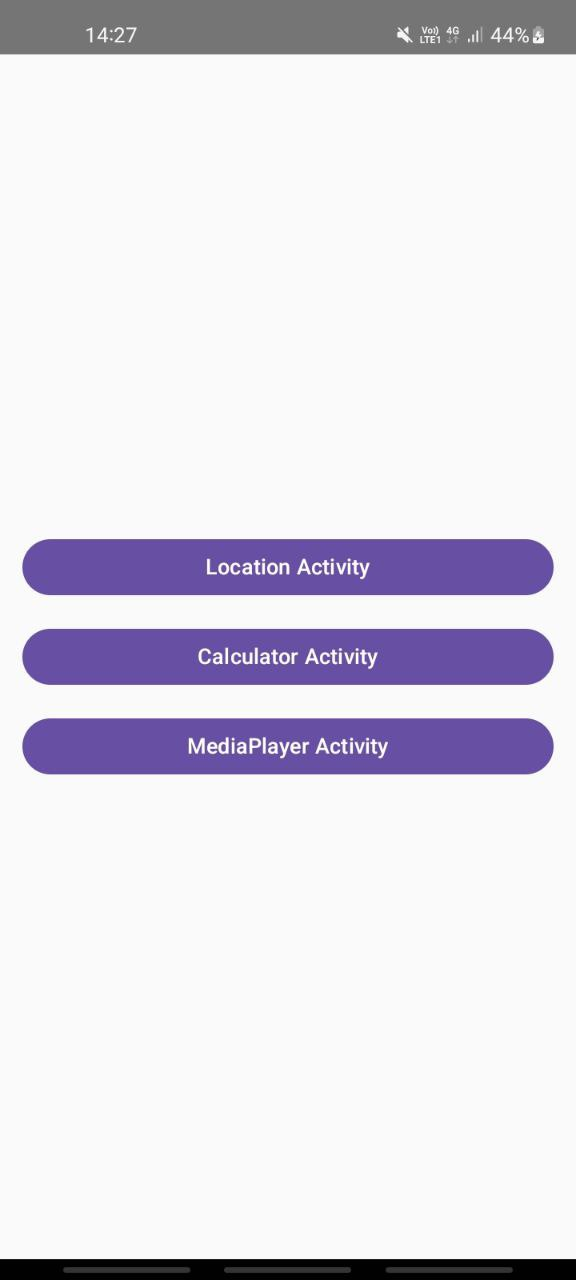
\includegraphics[width=0.5\textwidth]{1.jpg} % путь и размер
    \caption{}
    \label{fig:myimage1}
\end{figure}

\begin{figure}[h] % h – размещение "здесь"
    \centering
    
\includegraphics[width=0.5\textwidth]{2.jpg} % путь и размер
    \caption{}
    \label{fig:myimage2}
\end{figure}


\begin{figure}[h] % h – размещение "здесь"
    \centering
    
\includegraphics[width=0.5\textwidth]{3.jpg} % путь и размер
    \caption{}
    \label{fig:myimage3}
\end{figure}

\printbibliography[title=Список использованных источников] % Автособираемый список литературы

\end{document}